\documentclass[tikz,border=3pt]{standalone}
\usepackage{tikz-feynman}
\begin{document}
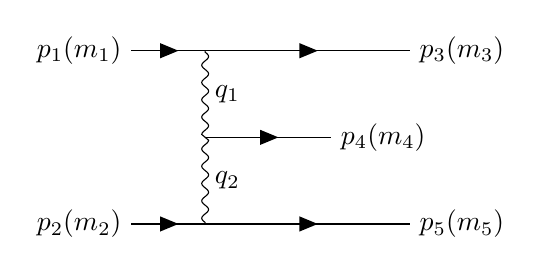
\begin{tikzpicture}
\begin{feynman}
\vertex (p1) {\(p_1(m_1)\)};
\vertex[right=1.6cm of p1] (A);
\vertex[right=2.6cm of A] (p3) {\(p_3(m_3)\)};
\vertex[below=2.2cm of p1] (p2) {\(p_2(m_2)\)};
\vertex[right=1.6cm of p2] (B);
\vertex[right=2.6cm of B] (p5) {\(p_5(m_5)\)};
\vertex[right=2.6cm of A, below=1.1cm of A] (C);
\vertex[right=1.6cm of C] (p4) {\(p_4(m_4)\)};

\diagram* {
  (p1) -- [fermion] (A) -- [fermion] (p3),
  (p2) -- [fermion] (B) -- [fermion] (p5),
  (A) -- [photon, edge label=\(q_1\)] (C),
  (B) -- [photon, edge label'=\(q_2\)] (C),
  (C) -- [fermion] (p4),
};
\end{feynman}
\end{tikzpicture}
\end{document}
